\documentclass[a4paper, twocolumn, 11pt]{beamer}

\usetheme{Darmstadt}
\usefonttheme[onlylarge]{structurebold}
\setbeamerfont*{frametitle}{size=\normalsize,series=\bfseries}
%\setbeamertemplate{navigation symbols}{}

\usepackage[cp1250]{inputenc}
\usepackage[english]{babel}
\usepackage{times}
\usepackage[T1]{fontenc}
\usepackage{pgf}
\usepackage{tikz}
\usepackage{listings}

\newcommand{\jmltobmltext}{JML2BML}
\newcommand{\jmltobml}{\textsl{\jmltobmltext}\xspace}
\newcommand{\openjml}{OpenJML\xspace}
\newcommand{\bmllib}{BMLLib\xspace}

\lstdefinelanguage{BML}{morekeywords={abstract,break,byte,case,catch,char,class,%
      const,continue,default,do,double,else,extends,false,final,%
      finally,float,for,goto,if,implements,import,instanceof,%
      interface,label,long,native,new,
      boolean, int,%
      null,%
      package,private,protected,public,ghost,%
      return,short,static,super,switch,synchronized,this,throw,%
      throws,transient,true,try,void,volatile,while,
      requires,precondition,ensures,exsures,exists,forall,&&,%
      old_this,loop_inv,\result,\everything,\nothing,%
      loop_specification,modifies,invariant,decreases,%
      iconst_0,iconst_1,istore_3,iinc,iload_3,%
      aaload,aload_0,aload_1,aload_2,aastore,%
      if_acmpne,if_icmplt,%
      invokespecial,getfield,%
      arraylength,ireturn},%
   sensitive,%
   morecomment=[l]//,%
   morestring=[b]",%
   morestring=[b]',%
    basicstyle=\scriptsize,
    keywordstyle=\bfseries\color{black},
    commentstyle=\itshape\color{blue},
    mathescape=true,
}

\title{Supplementing Java Bytecode with Specifications}
\author[Fulara, Jakubczyk, Schubert]{%
  J�drzej~Fulara \and
  Krzysztof~Jakubczyk \and
  Aleksy~Schubert \and
}
\institute{
Institute of Informatics\\
University of Warsaw\\
ul. Banacha 2\\
02-097 Warsaw, Poland
}
\date[CEE-SET 2008]{3rd IFIP TC2 Central and East European Conference on Software Engineering Techniques}

\begin{document}

\begin{frame}
\titlepage
\end{frame}

\begin{frame}{Outline}
  \tableofcontents
\end{frame}

\section{Introduction}

\subsection{Security of programs}

\begin{frame}{Problem}
  \begin{block}{We want programs to be}
    \begin{itemize}
    	\item Secure
    	\item Trustworthy
    	\item Bug-free
    \end{itemize}
  \end{block}
  \pause
  \begin{block}{Currently security is obtained by}
    \begin{itemize}
    	\item Bytecode verification
    	\item Digital certificates
    	\item Statical code analysis
    	\item Runtime checking
    \end{itemize}
  \end{block}
\end{frame}

\subsection{Proof-Carrying Code}

\begin{frame}{Idea}
	\begin{block}{Goal}
		Give the user certain guarantees of the code to be executed at the moment of its execution.
	\end{block}
	
	\pause
	
	\begin{block}{Solution}
		Augmented executable code with a proof that the code obeys certain policies.
	\end{block}
\end{frame}

\begin{frame}{PCC architecture for bytecode}
\begin{figure}
\begin{center}
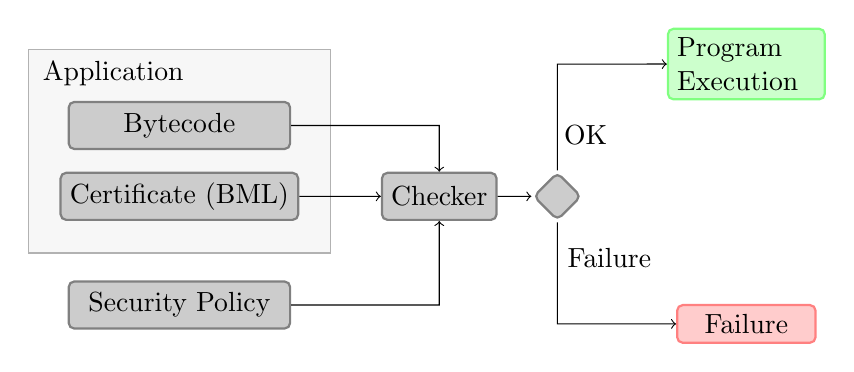
\begin{tikzpicture}[scale=0.6]

\tikzstyle{vertex}=[rectangle,draw=black!50,fill=black!20,thick,rounded corners = 2pt, minimum width=80pt, minimum height=17pt]
\tikzstyle{vertex2}=[rectangle,draw=black!50,fill=black!20,thick,rounded corners = 2pt, minimum height=17pt]
\tikzstyle{vertex3}=[rectangle,draw=green!50,fill=green!20,thick,rounded corners = 2pt, minimum width=55pt, text width=50pt]
\tikzstyle{vertex4}=[rectangle,draw=red!50,fill=red!20,thick,rounded corners = 2pt, minimum width=50pt]

\tikzstyle{rotated}=[rectangle,draw=black!50,fill=black!20,thick,rounded corners = 2pt,rotate=45, minimum height=12pt, minimum width = 12pt]
\tikzstyle{rl}=[line join = round]
\filldraw[draw=black!30,fill=black!3] (-3.2,3.8) rectangle (3.2,-0.5);
\node (app) at(-1.4,3.3) {Application};
\node[vertex] (bytecode) at (0,2.2){Bytecode};
\node[vertex] (certificate) at (0,0.7) {Certificate (BML)};

\node[vertex](policy) at (0, -1.6) {Security Policy};

\node[vertex2](checker) at (5.5,0.7) {Checker};
\node[rotated](rot) at (8, 0.7) {};
\node[vertex3](execution) at (12,3.5) {Program Execution};
\node[vertex4](failure) at (12,-2) {Failure};
\draw[->] (certificate) to[out=0,in=180] (checker);
\draw[->] (checker.east) -- (7.45,0.7);
\draw[->] (bytecode.east) -- (5.5,2.2) -- (checker.north);
\draw[->] (policy.east) -- (5.5,-1.6) -- (checker.south);
\draw[->] (8,1.25) -- (8,3.5) -- (execution.west);
\draw[->] (8,0.15) -- (8,-2) -- (failure.west);
\node (ok) at (8.6, 2) {OK};
\node (ok) at (9.1, -0.6) {Failure};
\end{tikzpicture}
\end{center}
\end{figure}
\end{frame}

\begin{frame}{PCC infrastructure}
\begin{itemize}
	\item checker tools for BML annotations combined with PCC certificates
	\item tools which enable the construction of PCC certificates
	\item procedures to safely distribute the desired properties to be checked by PCC infrastructure
	\item modeling languages (such as JML) for other programming languages
	\item<1->\alert<2> {compilers that transform programs to JVM bytecode with annotations}
\end{itemize}
\end{frame}

\section{Background}

\subsection{Java Modeling Language}

\begin{frame}[fragile]
	\frametitle{What is JML?}

		\begin{itemize}
			\item behavioural specification language for Java
			\item write specifications in \emph{design-by-contract} fashion
		\end{itemize}

\end{frame}

\begin{frame}[fragile]
	\frametitle{JML example}
	
\lstset{language=java, morekeywords={requires,ensures,\result,\exists,\old,loop_invariant,\forall,==>, decreases},
        basicstyle=\tiny,commentstyle=\tiny,moredelim=*[s][\tiny]{/*@}{*/},
        numbers=left,numberstyle=\tiny,stepnumber=2,numbersep=4pt}
\begin{lstlisting}
public class List {

  private Object[] list;

  /*@ requires list != null;
    @ ensures \result ==(\exists int i;
    @ 0 <= i && i < list.length &&
    @ \old(list[i]) == o1 && list[i] == o2);
    @*/
  public boolean replace(Object o1, Object o2){
    /*@
      @ loop_invariant i <= list.length
      @ && i >=0 && (\forall int k;0 <= k
      @ && k < i ==> list[k] != o1);
      @ decreases list.length - i;
      @*/
    for (int i = 0; i < list.length; i++) {
      if (list[i] == o1) {
        list[i] = o2;
        return true;
      }
    }
    return false;
  }
}
\end{lstlisting}	

\end{frame}

\subsection{Bytecode Modeling Language}

\begin{frame}[fragile]
	\frametitle{What is BML?}

		\begin{itemize}
			\item specification language for Java bytecode
			\item design of BML directly follows the fundamental concepts of JML
			\item BML is developed within the MOBIUS project
			\item target of the project are Java-enabled mobile devices
			\item current version of BML assumes some simplifications of the Java bytecode which are present in the J2ME mobile platform
			\item Class files with BML annotations are regular Java class files
			\item annotations are stored within additional attributes
			\item attributes start with the prefix \emph{org.bmlspecs} and according to the specification of JVM they should be ignored in normal execution
			\item Following the logical structure of class files, class specifications are stored as class attributes, method specifications, as method attributes and specifications inserted in the bytecode are subattributes of the JVM Code attributes.
		\end{itemize}

\end{frame}

\begin{frame}[fragile]
	\frametitle{BML example}

\begin{figure}[htb]
\lstset{language=bml}
\lstset{basicstyle=\scriptsize,stepnumber=400,numbersep=5pt}
\vspace{-2\baselineskip}
~\hspace{2cm}~\begin{minipage}{400pt}
\begin{lstlisting}
/*@
  @ requires this.list != null
  @ ensures \result ==
  @   (\exists int i; 0 <= i &&
  @            i < this.list.length &&
  @            old_this.list[i] == o1 &&
  @            this.list[i] == o2)
  @*/
public boolean replace(Object o1, Object o2)
0:    iconst_0
1:    istore_3
2:    goto	   #27
5:    aload_0
6:    getfield	   main.List.list
9:    iload_3
10:   aaload
11:   aload_1
12:   if_acmpne	   #24
15:   aload_0
16:   getfield	   main.List.list
19:   iload_3
20:   aload_2
21:   aastore
22:   iconst_1
23:   ireturn
24:   iinc	   %3	1
27:   iload_3
28:   aload_0
29:   getfield	   main.List.list
32:   arraylength
/*@
  @ loop_specification
  @   modifies everything
  @   invariant i <= this.list.length &&
  @      i >= 0 &&
  @      (\forall int k; 0 <= k &&
  @          k < i ==> this.list[k] != o1)
  @   decreases this.list.length - i
  @*/
33:   if_icmplt	   #5
36:   iconst_0
37:   ireturn
\end{lstlisting}
\end{minipage}


\caption{The method \texttt{replace} in the \texttt{List.class}}
\label{fig:bytecode}
\end{figure}
\end{frame}

\section{Jml2Bml Compiler}
\subsection{What is it?}

\begin{frame}{In General}
	\begin{block}{What it does?}
		Jml2Bml compiler translates JML annotations to BML annotations.
	\end{block}
	\begin{block}{Input}
		\begin{itemize}
			\item Java source file with JML annotations
			\item corresponding class file
		\end{itemize}
	\end{block}
	\begin{block}{Output}
		\begin{itemize}
			\item class file with proper BML annotations inserted
		\end{itemize}
	\end{block}
\end{frame}

\subsection{Design}
\begin{frame}{In General}
	\begin{block}{Key Features}
	  \begin{itemize}
	  	\item acyclic structure of modules
	  	\item uses enhanced Abstract Syntax Tree from OpenJML compiler
	  	\item separate translation rules for JML nodes
	  	\item translation rule applied at each node of the AST
	  	\item succeessfull translation result is stored in output class file using BMLLib library
	  \end{itemize}
	\end{block}
  
  \pause
  
  \begin{block}{Advantages of the design}
  	\begin{itemize}
  		\item easily extensible
  		\item compatible with Umbra bytecode tool
  	\end{itemize}
  \end{block}
\end{frame}

\begin{frame}{Translation mechanism}
	\begin{block}{Translation rule}
		\begin{itemize}
			\item compiler uses a set of translation rules
			\item each responsible for a relatively small piece of translation
		\end{itemize}
	\end{block}
	\pause
	\begin{block}{Key design features}
		\begin{itemize}
			\item the concept falls into a visitor design pattern
			\item translation rule is an extension of a simple abstract class
			\item translation process can be broken into smaller, independent pieces
			\item extending translation is simple
		\end{itemize}
	\end{block}
\end{frame}

\subsection{Loopa}
\begin{frame}
	co� o p�tlach
\end{frame}

\subsection{Application}
\begin{frame}
	zastosowanie
\end{frame}

\section*{Summary}

\begin{frame}
  \frametitle<presentation>{Summary}
  
	\begin{block}{Jml2Bml compiler is}
		\begin{itemize}
			\item tool that translates annotations from JML to BML
			\item part of PCC infrastructure
			\item easily extensible
		\end{itemize}
	\end{block}

\end{frame}

\end{document}
